\section{Análisis de resultados integrales}

En este capítulo, se presentan los resultados integrales de nuestra investigación, que se centra en dos aspectos cruciales para la optimización de la gestión de recursos en sistemas operativos. En primer lugar, introduciremos los resultados del módulo de Encendido y Apagado de Procesadores. En segundo lugar, se presentarán los del módulo de Monopolización de Núcleos.\par

Ambos mecanismos desarrollados proporcionan al sistema operativo y a la red las herramientas necesarias para mejorar la gestión de sus recursos. Es fundamental tener presente que estos mecanismos representan un paso esencial hacia la consecución de objetivos más amplios, específicamente relacionados con mejoras en la eficiencia energética y el rendimiento general del sistema. La exposición de resultados tiene como objetivo destacar la funcionalidad adecuada de la implementación de los módulos previamente desarrollados en este informe, acercándonos a  los objetivos más amplios mencionados.\par

Como se detalló en la sección de desarrollo de este informe, previo a  la implementación de los módulos mencionados llevamos a cabo una actualización del código del kernel, para incorporar al último lanzamiento estable de FreeBSD, las modificaciones realizadas en el proyecto integrador previo. Decidimos incluir los resultados de esta actualización al final de este capítulo, dado que consideramos que los módulos son más propensos a un análisis detallado y a comprender sus resultados. En contraste, las actualizaciones simplemente requieren que el sistema continúe funcionando correctamente.\par

% TODO{ESCRIBIR ALGO SOBRE LAS HERRAMIENTAS QUE SE IMPLEMENTARAN A LA HORA DE LOS ANÁLISIS.}


\subsection{Resultados de la Implementación del Módulo de Encendido/Apagado de Procesadores}
La implementación del módulo de encendido/apagado de procesadores en FreeBSD, utilizando el enfoque de Redes de Petri, se realizó como punto de inicio del camino hacia la mejora de eficiencia y gestión de recursos del sistema operativo. En esta sección, presentaremos los resultados obtenidos de nuestras pruebas y analizaremos cómo este módulo afecta el rendimiento del sistema.\par


\subsubsection{Estado Inactivo del Sistema}
En situaciones de inactividad del sistema operativo, caracterizadas por la ausencia de tareas pendientes, cada procesador opera en un modo especial ejecutando hilos de la clase IDLE. Este escenario está diseñado para que el sistema mantenga un estado pasivo, preparado para abordar de manera eficiente cualquier tarea que pueda emerger.\par

Creemos importante resaltar que, independientemente de si nuestro módulo de encendido/apagado está activo para alguno de los procesadores en este contexto, hemos considerado y abordado esta situación en nuestra implementación para garantizar la estabilidad del sistema. La Figura \ref{fig:cpuOnOff-load-inactive} proporciona una representación visual de este estado.\par

\begin{figure}[H]
    \centering
    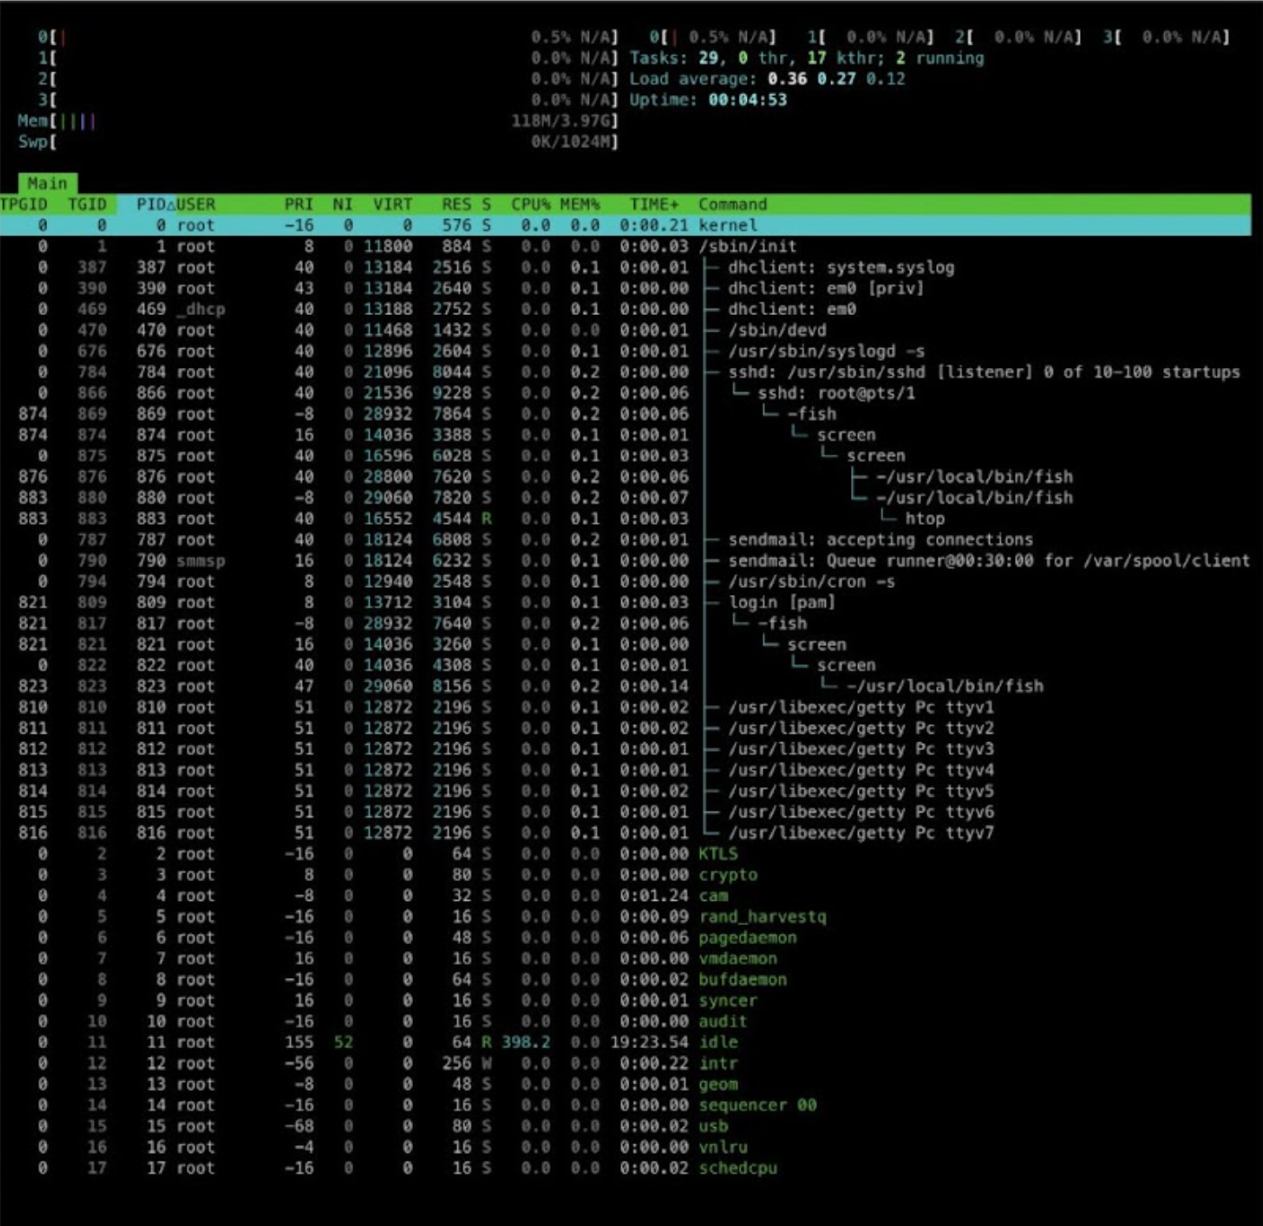
\includegraphics[width=0.8\textwidth]{images/cpuOnOff-load-inactive.png}
    \caption{Estado inactivo del sistema.}
    \label{fig:cpuOnOff-load-inactive}
\end{figure}

\subsubsection{Comportamiento con el Módulo Inhabilitado}
Cuando el módulo de encendido/apagado de procesadores no está habilitado para ningún núcleo, el sistema operativo sigue su funcionamiento convencional bajo la lógica del planificador. En este estado, el \textit{scheduler} opera mediante el uso de la Red de Petri  con las plazas y transiciones de cada uno de los procesadores del sistema, sin hacer uso de la adición de plazas y transiciones que corresponden al módulo, introducidas en el desarrollo del mismo.\par

Para confirmar dicho comportamiento, llevamos a cabo una prueba de estrés sobre los procesadores, ejecutando un programa que genera múltiples procesos que realizan cálculos matemáticos complejos. Durante la ejecución del programa, supervisamos el sistema y observamos que todos los procesadores operaban al máximo de su capacidad, funcionando al 100\% para completar la tarea. La Figura \ref{fig:cpuOnOff-load-disabled} proporciona una representación visual de este estado.\par

Este escenario de funcionamiento con el módulo deshabilitado proporciona un punto de referencia inicial para comprender el impacto de nuestra implementación en la gestión de recursos y el rendimiento general del sistema operativo.\par

\begin{figure}[H]
    \centering
    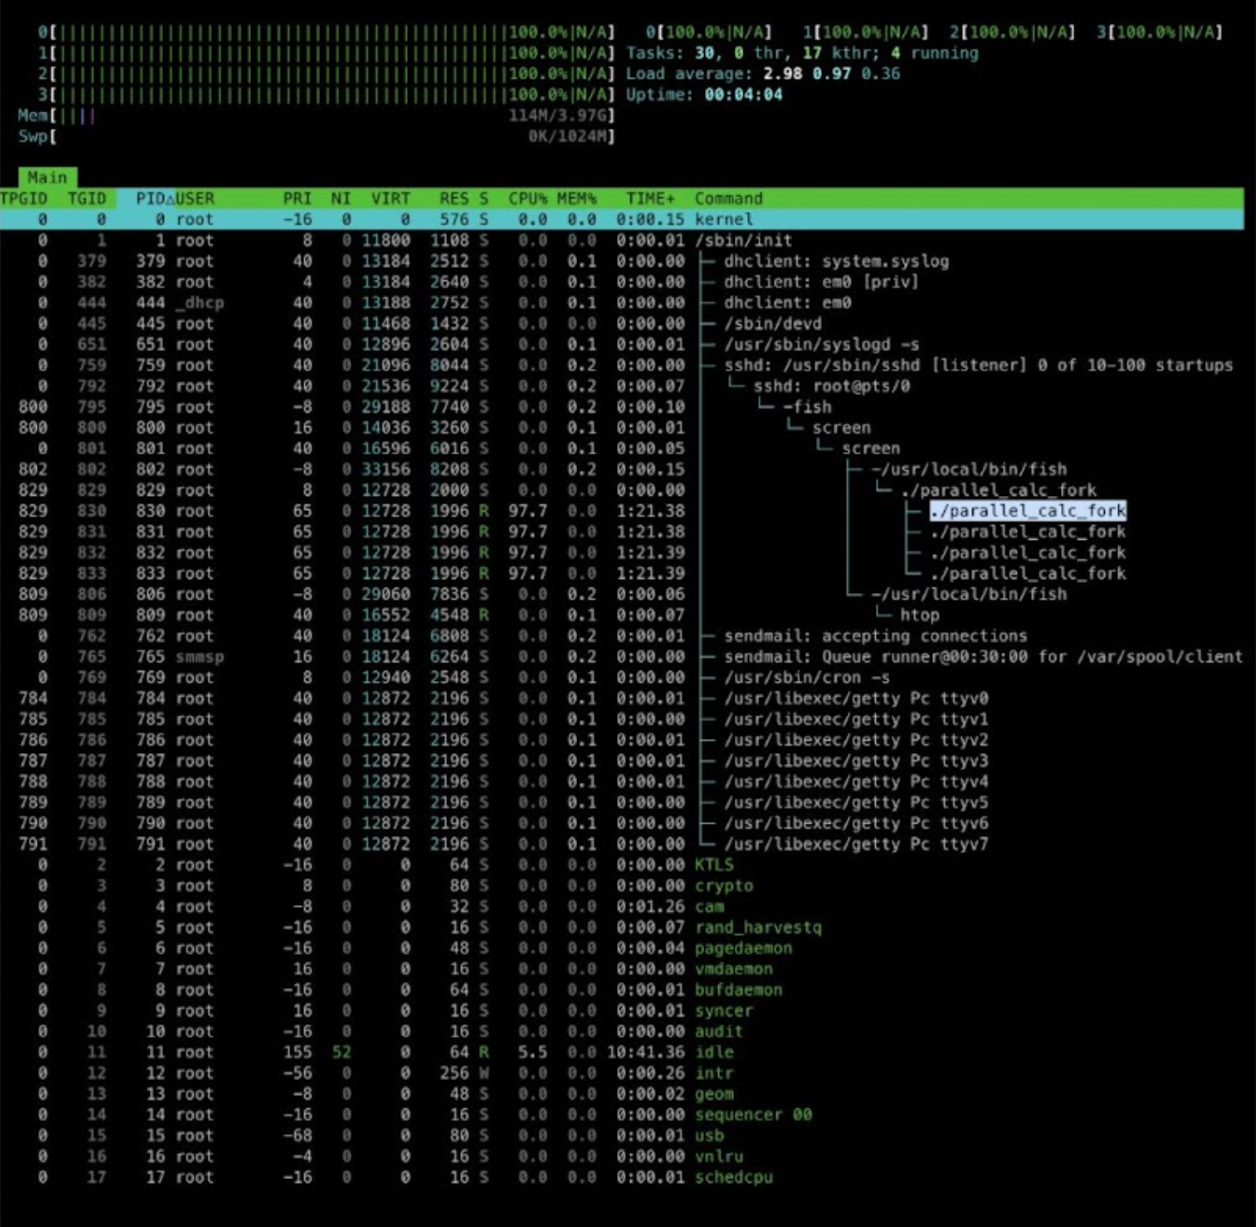
\includegraphics[width=0.8\textwidth]{images/cpuOnOff-load-disabled.png}
    \caption{Estado de los núcleos con el modulo encendido/apagado inhabilitado.}
    \label{fig:cpuOnOff-load-disabled}
\end{figure}

\subsubsection{Comportamiento con el Módulo Habilitado}
Basándonos en las observaciones anteriores, llevamos a cabo la misma prueba de estrés, pero activando previamente el módulo de encendido/apagado para inhabilitar el Procesador 2.\par

Este enfoque nos permitió no solo corroborar la funcionalidad adecuada de la implementación, sino también analizar la respuesta del sistema ante un cambio tan significativo como el bloqueo del encolado en uno de sus núcleos.\par

En relación a los resultados obtenidos durante esta evaluación, observamos que, al suspender uno de los procesadores del sistema, este continuó funcionando de manera estable. Se puede apreciar que la carga del procesador suspendido se mantuvo en cero, mientras que los demás procesadores continuaron ejecutando los cálculos. Esto demuestra de manera concluyente que el sistema fue capaz de adaptarse sin dificultades a la reducción de recursos de procesamiento.\par

% TODO{IMAGEN CON PROCESADOR SUSPENDIDO}

En relación al tiempo necesario para completar el cálculo del programa, notamos que dicho tiempo aumentó proporcionalmente a la disminución en el número de procesadores activos, destacando la correlación entre la disponibilidad de recursos de procesamiento y el tiempo total requerido para finalizar el programa. En la % TODO{FIGURA TANTO} podemos comprobar el funcionamiento del sistema con la inhabilitación simultánea de dos procesadores.\par

% TODO{IMAGEN CON DOS PROCESADORES SUSPENDIDOS}

% TODO{TABLA CON LOS TIEMPOS DE EJECUCION CON TODOS LOS PROC, CON 3 Y CON 2 + explicacion + diciendo que el objetivo no es tener apagos los procesadores en tiempos de estres, sino que se muestra solo para ejemplificar, y que la parte del kernel que en un futuro haga uso del modulo para reducir los gastos energeticos, tiene que entender cuando conviene apagar. (Medio como conclusion del modulo)}

% TODO{branch con el codigo}


\subsection{Resultados del módulo de Monopolización de Núcleos}
La implementación del módulo de Monopolización de Núcleos en FreeBSD constituyó el próximo paso en el desarrollo de este proyecto integrador. A continuación, se expondrán en detalle los resultados alcanzados al concluir dicho módulo.\par
\subsubsection{Estado Normal del Sistema}
En este apartado se analizará el comportamiento general del sistema con el módulo de monopolización deshabilitado. Es relevante señalar que bajo esta configuración, los procesadores operan de forma predeterminada, utilizando la Red de Petri como planificador para mantener el equilibrio de la carga. De esta forma, los núcleos que en algún momento carezcan de tareas tomarán hilos de la cola global o ejecutaran hilos de clase IDLE en caso de inactividad del sistema.\par

% TODO{ENCONTRAR UNA FORMA DE MOSTRAR COMO LOS HILOS SE PLANIFICAN SIN TENER EN CUENTA LA MONOPOLIZACION, CAMBIANDO SU EJECUCION ENTRE LOS DISTINTOS NUCLEOS}


\subsubsection{Comportamiento con el Módulo Habilitado}
Habiendo expuesto el comportamiento del sistema en su condición normal, se sienta una base para la posterior comparación con el desempeño del módulo.\par

Siguiendo un procedimiento similar al empleado con el módulo de encendido y apagado, procedimos a ejecutar el programa de estrés, orientado al cálculo de números primos. Durante su ejecución, la herramienta de monitoreo (htop) permite la observación de los distintos subprocesos vinculados a este programa y la información específica de cada uno, incluyendo el identificador de cada hilo, el cual adquiere relevancia antes de activar el módulo.\par

En este momento, nos enfocamos en los procesadores que ejecutan cada subproceso y cómo pueden variar según las decisiones del planificador.

% TODO{2 imágenes con los subprocesos, que se pueda ver una comparación de cómo cambia el CPU para alguno de los subprocesos, es decir, subproceso 1 primer imagen corre en el cpu 1, segunda imagen ese mismo subproceso corre en cpu 3}

Con el programa en ejecución y el monitoreo activado, el siguiente paso implica la configuración del módulo; en otras palabras, es el momento de actualizar las variables dentro del código del módulo. La primera variable a considerar es el identificador del subproceso que deseamos anclar a un núcleo específico, obtenido previamente del programa de monitoreo. Una vez que tenemos el identificador, procedemos a seleccionar en qué núcleo asociaremos este hilo, compilando y cargando el módulo de kernel adecuado.\par

Los resultados obtenidos concuerdan con la información proporcionada por la  herramienta de monitoreo. En este caso, hemos seleccionado el hilo con el identificador  878172 y el CPU 2. Como era de esperar, tras la ejecución del módulo, este subproceso estuvo vinculado al CPU durante toda su ejecución. Además, ningún otro hilo o proceso se ejecutó en ningún momento en este núcleo, evidenciando así su exclusividad y el correcto funcionamiento del desarrollo.\par

% TODO{Imagen con el hilo asociado al núcleo, quizás también podemos tener un link a video para mostrar hasta que termina de ejecutarse, y con la desactivación del módulo para ver como el cpu vuelve a estar disponible para los otros procesos}

Un caso relevante es el estado del sistema una vez que el programa de estrés ha concluido pero el módulo permanece activado. En estas condiciones, se puede observar cómo el CPU al que se había anclado el hilo permanece “reservado”, sin ejecutar ningún hilo que no posea el ID especificado, mientras que los procesos restantes solo se ejecutan en los núcleos liberados. Con esto en mente, se puede identificar una similitud con el funcionamiento del módulo de encendido/apagado al desactivar un núcleo.\par

Al desactivar el módulo, el sistema continúa operando según lo esperado, con todos sus núcleos disponibles, tal como lo haría en su estado normal.

% TODO{branch con el codigo}

\subsection{Resultados de las actualizaciones en la versión del S.O.}
En esta sección, se expondrán los resultados derivados de las actualizaciones implementadas en el marco del proyecto integrador previo. Es relevante subrayar que estas actualizaciones se llevaron a cabo con el propósito de sincronizar el proyecto con la versión más reciente y estable del sistema operativo (versión 13.1). Dado que la implementación original demostró su eficacia en la versión 11, el énfasis principal en esta sección se dirigirá a garantizar la continuidad de dicho rendimiento.\par

Esta fue la primera tarea abordada en este proyecto, y la elección de priorizarla desde el inicio se fundamentó en la necesidad de mantenerse alineado con la comunidad y acceder a posibles recursos de apoyo cuando fuese necesario. Asimismo, esta estrategia facilitó el desarrollo sobre una base de código más actualizada, evitando conflictos significativos que pudieran surgir en fases finales del desarrollo.\par

A pesar de la necesidad de revisar numerosos conflictos generados entre el código del planificador en la versión 11 y la versión 13 de FreeBSD, los resultados finales obtenidos de esta etapa confirman que la actualización se realizó con éxito. El sistema operativo, con el planificador de redes de Petri, mantuvo la estabilidad y el funcionamiento adecuado en las pruebas realizadas.\par

El código correspondiente a esta etapa se encuentra en una rama específica del repositorio del proyecto. Debido a la estructura de ramas y modalidad de trabajo que se planteó para la realización de este trabajo integrador, también podemos encontrar una rama por cada actualización que se fue realizando progresivamente desde la 11 hasta la 13.1.\par

% TODO{MOSTRAR ALGUNAS IMAGENES DEL PROYECTO CORRIENDO CON LA VERSION 13.1 Y UTILIZANDO LA RED}

\subsection{Resultados del tareas extra % TODO{OPCIONAL - VER SI LO AGREGAMOS}}

